
%%%%%%%%%%%%%%%%%%%%%%%%%%%%%%%%%%%%%%%%%%%%%%%%%%%%%%%%%%%%%%%%%%%%%%%%
\chapter{Spacial Analysis} \label{chap_spacial}
%%%%%%%%%%%%%%%%%%%%%%%%%%%%%%%%%%%%%%%%%%%%%%%%%%%%%%%%%%%%%%%%%%%%%%%%

%%%%%%%%%%%%%%%%%%%%%%%%%%%%%%%%%%%%%%%%%%%%%%%%%%%%%%%%%%%%%%%
\section{Introduction to Spacial Analysis} \label{sec_intro_spac}

% note difference between last section and this section, were gonna focus a lot more on environment os buckle up
In \autoref{sec_probsnstat}, ambient noise was split into three distinct acoustic environments in order to asses the overall attributes of each. With the numerical attributes of each environments differing by frequency, it is likely the causes and drivers of this ambient noise differ as well. Acoustic forces behind sound under ice are not the same as the primary powers behind sound in an ice free Arctic ocean. This section will focus on the relationship between ambient sound under ice and the movement of ice itself.

A significant amount of this section is a continuation of the work done in a previous iteration of the data in \footcite[]{BonnelMain}. The focus here is exclusively on the ambient noise when ice is present, and does not divide between 'ice with duct' and 'ice without duct' like in \autoref{sec_probsnstat}. The entire time period encompassed by this section is from 01NOV2016 to 30JUL2017, but the highest correlations occurring from 1DEC2016 to 30MAY2017. Time periods with low quality ice data were omitted. Expanding the frequencies examined in spacial correlation analysis emphasizes that all these frequencies are highly related in both sound level, perhaps due to driving source of ice drift. 

While looking at a broadband range of frequencies makes sense for a statistical analysis, looking at the spatial correlation of 38 different frequencies on a map would be cluttered. For ease of computing and viewing, the spatial correlation analysis is limited to the frequencies of 300 Hz, 500 Hz, 1000 Hz, and 1500 Hz. Each band was 50 Hz wide, echoing the conventions of \autoref{sec_probsnstat}. 300 Hz, as opposed to 250 Hz, was retained for comparison with the original analysis; it is known from \autoref{sec_probsnstat} that 250 Hz and 300 Hz are closely related anyhow. While a band around 50 Hz was examined, the low frequencies behaved more erratically than all the other frequencies. This is reflected in the statistic analysis above as the 50 Hz data points are usually different and and it could be assumed the low frequencies have different acoustic drivers. 

%%%%%%%%%%%%%%%%%%%%%%%%%%%%%%%%%%%%%%%%%%%%%%%%%%%%%%%%%%%%%%%%%%%%%%%%
% seriously why do all my titles sound terrible
\section{Spacial Analysis Methods and Results}
%%%%%%%%%%%%%%%%%%%%%%%%%%%%%%%%%%%%%%%%%%%%%%%%%%%%%%%%%%%%%%%%%%%%%%%%


%%%%%%%%%%%%%%%%%%%%%%%%%%%%%%%%%%%%%%%%%%%%%%%%%%%%%%%%%%%%%%%%%%%%%%%%%%
\subsection{Spacial Correlation between Ice Drift and ANL Method} \label{sec_corr_method}

As described in \autoref{intro_env_info}, the time periods over which the variables of ambient noise and ice drift movement (IDM) are 7 minutes and 24 hours respectively. To make the two comparable, ANL was decimated to match the sampling rate of the IDM. As, the exact metrics of ANL and ice drift cannot be directly compared due to their different units. Normalized values for both variables were computed using z-scores and then correlated over specific time periods. 

Correlation was calculated at each point of the IDM map for a 2 month long period of time centered on $t_{0}$; each 2 month long time period center is separated by two weeks, leading to sliding windows with 75\% overlap in time. \footcite[]{Bonnel2021} The equation to correlate these two metrics is 

\begin{equation}    \label{eq_spacialcorr}
    M(x,y,t_{0})=\Gamma [n(t_{0}),d(x,y,t_{0})]
\end{equation}
 
where $d(x,y,t_{0})$ represents the IDM time series for the time period centered on $t_0$, $M$ is the correlation map matrix, $x$ is longitude, $y$ is latitude, $n(t_0)$ is ANL during the 2 month long time period centered on $t_0$, and$\Gamma$ is the Pearson correlation function. Correlation coefficients with a $p>0.05$ were removed from the map. Correlations were calculated for various ANL frequencies using data from both SHRU1 and SHRU5, as discussed in \autoref{sec_corr_shru} and \autoref{sec_spa_corr_freqs}.%ref sections or not bc they all use this method

% describing how its plotted one time

For the figures of \autoref{sec_corr_shru} and \autoref{sec_spa_corr_freqs} the left column shows a colormap of the correlation coefficients. Land is included on the map for frame of reference. The red X represents the point of maximum correlation while the black X represents the position of the SHRU. Where the value of $p\leq0.05$ or if there is no IDM data, the map is white. 

Typically, the correlation color spread is centered on the red X, but isn't confined to one shape as seen in the bottom maps of \autoref{fig_300_16DEC} and \autoref{fig_1500_16DEC}. Distant dark spots on the lower end of the colorbar spectrum appear on some of the correlation maps like in \autoref{fig_300_500corr} and \autoref{fig_1000_1500corr}. These dark blue spots represent areas of low correlation where data was present and the p-value significant enough to not be rejected.

The right columns show the normalized time series of 2-day average ANL and IDM at the location of maximum correlation. The blue line is the ANL at that given frequency, which is more continuous than the orange line, which has ice drift per day. The maximum correlation value found between the ANL and ice drift is displayed at the top of each time series, corresponding with the red X of the map. Dates are displayed above the maps, as well as labels indicating where the correlation data came from, specific to each section.


%%%%%%%%%%%%%%%%%%%%%%%%%%%%%%%%%%%%%%%%%%%%%%%%%%%%%%%%%%%%%%%%%%%%%%%%%%5


%%%%%%%%%%%%%%%%%%%%%%%%%%%%%%%%%%%%%%%%%%%%%%%%%%%%%%%%%%%%%%%%%%%%%%%%%%
\subsection{Spacial Correlation across Frequencies} \label{sec_spa_corr_freqs}

\begin{figure}[p]
\centering
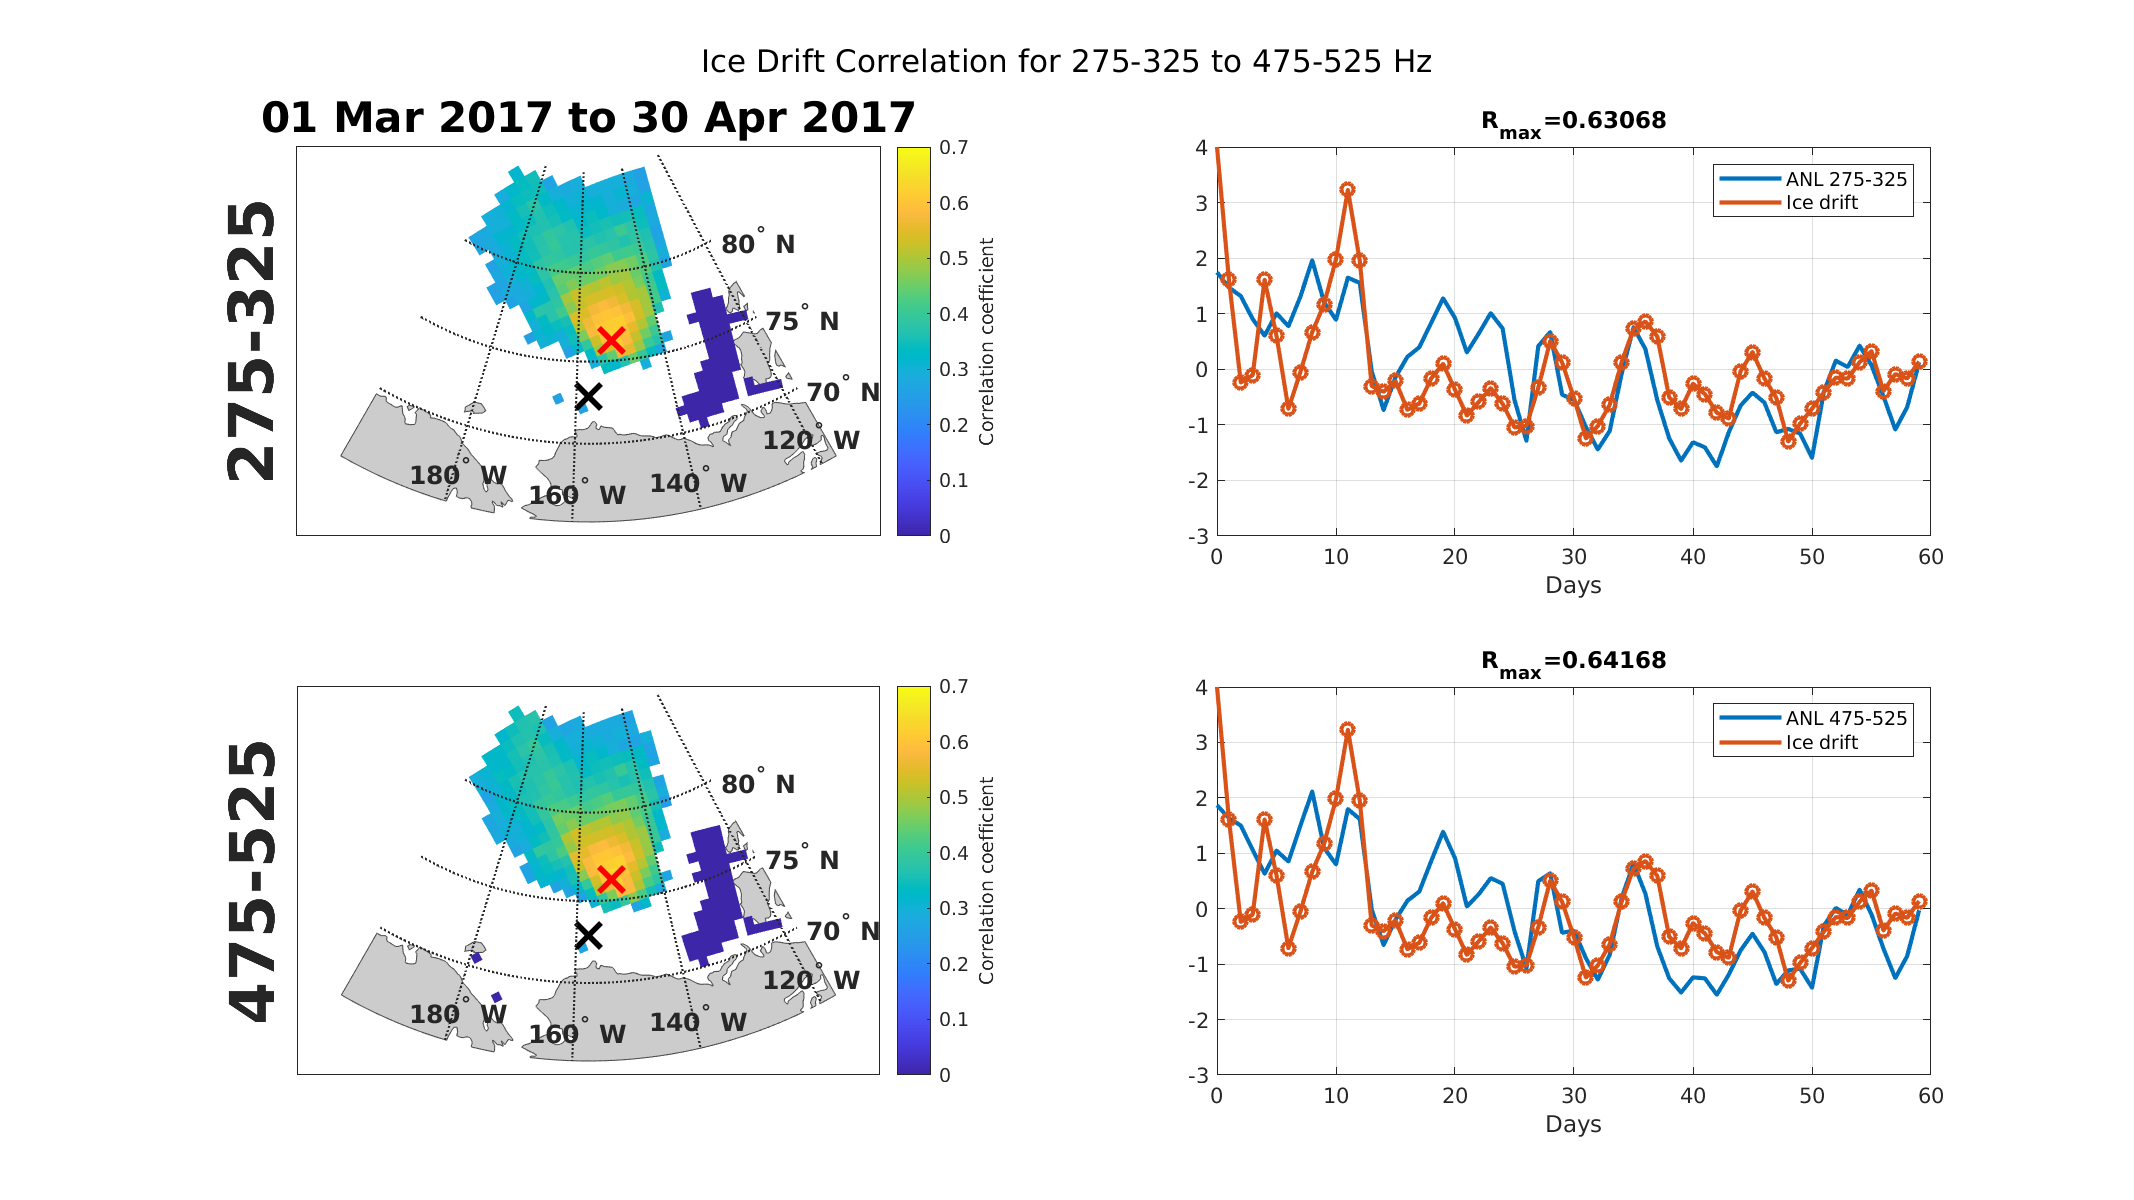
\includegraphics[scale=0.35]{Figures/300_500_spatial_corr_20170301-20170430.png}
\caption{Spacial Correlation map and time series from SHRU5 for 300 Hz and 500 Hz for March 1, 2017 to April 30, 2017}
\label{fig_300_500corr}
\end{figure}


\begin{figure}[p]
\centering
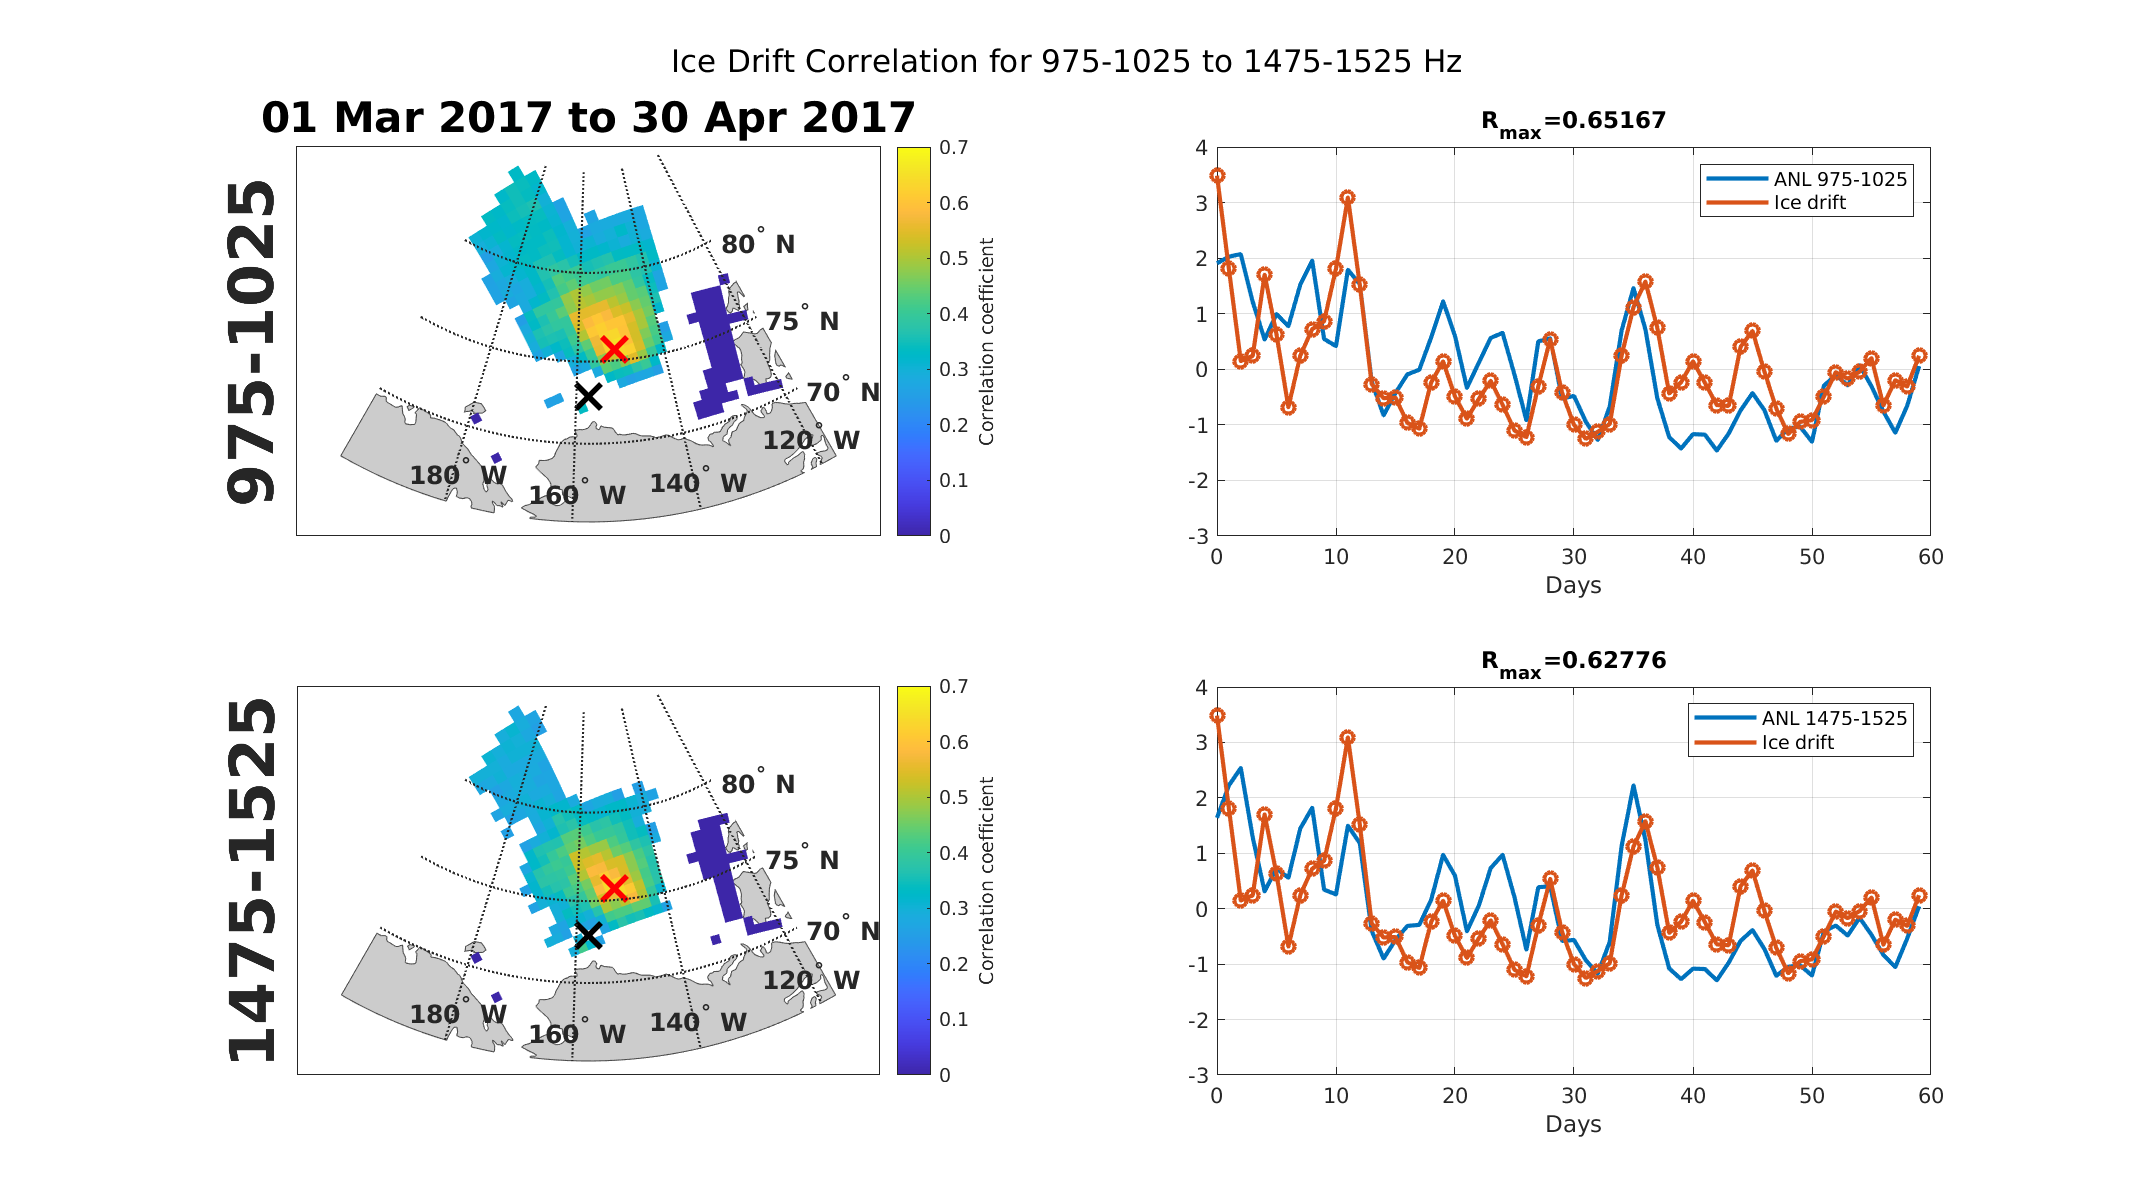
\includegraphics[scale=0.35]{Figures/1000_1500_spatial_corr_20170301-20170430.png}
\caption{Spacial Correlation map and time series from SHRU5 for 1000 Hz and 1500 Hz for March 1, 2017 to April 30, 2017}
\label{fig_1000_1500corr}
\end{figure}

Using the procedures as in the \autoref{sec_corr_method}, correlation maps and time-series for different frequencies were plotted together for direct comparison. To keep with \autoref{sec_probsnstat} and because it data seemed to have tighter colormaps, only data from SHRU5 was analyzed for the major frequencies of 300 Hz, 500 Hz, 1000 Hz, and 1500 Hz. The time period with the highest average correlation coefficient is displayed, but may have not been the actual maximum correlation for every frequency. \autoref{fig_300_500corr} and \autoref{fig_1000_1500corr} contain data from the period of March 1, 2017 to April 30, 2017, which is actually a period when the Beaufort Duct is not present \footcite[]{ballard2020yearlong}. Even without the helping presence of the Duct, long distance propagation is able to happen and picked up by hydrophones at the depth of the Duct. 

The normalized values of ANL and IDM have similar oscillations in time, with an exception on the fourth day where ANL increases but IDM does not. As theorized before, another environmental acoustic driver like an ice quake could be the cause for this spike in noise. Interestingly, 1000 Hz in \autoref{fig_1000_1500corr} had the highest correlation coefficient, followed by 500 Hz, 300 Hz, then 1500 Hz. From \autoref{sec_peak_prob}, peak probability ANL levels for 1500-300 Hz go from 55-69 dB. Even though sound levels reaching SHRU5 decreased 10 dB over frequency, maximum correlation values were not affected. The drift of the ice generating the sound at a distance creates matching ambient noise in a large breadth of frequencies recorded by the SHRU(s). 

All four spacial correlation colormaps have the same point of maximum correlation for this time period and a surrounding area of high (>0.4) correlation. The four also share the same block of minimal correlation from about 140 $\degree$ W to 120 $\degree$ W. Size and shape of the map's correlation spread differ for each frequency in . As frequency increases, the entire size of the colormap decreases. This decrease in correlation size could be due to the lower dB of ANL recorded for 1000 Hz and 1500 Hz, as  sound at higher frequency is likely to attenuate sooner. 

The map spread becomes more abstract in frequency, going from a contained block in \autoref{fig_300_500corr} to having a distended lobe on the northwest corner in \autoref{fig_1000_1500corr}. The area with correlation $>0.3$ in the 300 Hz map translates to the whole colormap of 1500 Hz, but 1500 Hz has lower correlation values. Maximum correlation value does not decrease, but the correlation map seems to be lower and darker in color as frequency increases. So while, strong correlation still exists between IDM and ANL, there are lower coefficients as frequency increases. Lower levels of ANL from sources and the distance sound must travel in the surface channel contribute to the decreasing amounts and values of correlation as frequency increases. Less correlation and lower values are likely due to the diminishing presence of 1000-1500 Hz ANL seen in \autoref{sec_probsnstat}.
% hahahah i keept saying blob until i remembered the word lobe exsits

When compared to December plots \autoref{fig_300_16DEC} and \autoref{fig_1500_16DEC} in the next section, the correlation output and maximum point have both shifted towards the east. This west to east drift of the IDM seems to move the sound source closer then further away from SHRU5, resulting in corresponding correlation coefficients. Looking at the movement of the correlation spread in time across frequencies shows similar patterns, further explored in \autoref{sec_allfreq_map}.

% can probably shave down figure sides to make bigger if needed

%%%%%%%%%%%%%%%%%%%%%%%%%%%%%%%%%%%%%%%%%%%%%%%%%%%%%%%%%%%%%%%%%%%%%%%%%%%%
\subsection{Spacial Correlation across SHRU(s)} \label{sec_corr_shru}

This section uses the same procedures as in \autoref{sec_corr_method} and used above for \autoref{sec_corr_shru}. Ambient noise and IDM correlation exists across hydrophones in the array \autoref{fig_location}, but correlation values differs due to the different geographic location of SHRU5 and SHRU1. Two figures are shown demonstrating the correlation between SHRU(s) for different times, created using the methods specified in \autoref{sec_corr_method}. Results from SHRU5 are plotted on the top row, and results from SHRU1 are plotted on the bottom row. 

\autoref{fig_300_16DEC} is a replica of the original 300 Hz examined in the preliminary study \footcite[]{Bonnel2021} but shown at a different date. \autoref{fig_1500_16DEC} focuses on a frequency band centered around 1500 Hz, as opposed to 300 Hz. In \autoref{sec_corr_freq}, it was definitively shown that ambient noise is highly related through a wide swathe of frequencies. These correlation plots for two distant frequencies reflect this theory for both hydrophones. From this, it can be inferred that ambient noise under ice is similar in frequency and space, as these distant, separate hydrophones show similar correlations.   % wanted both to prove the matching across time

\begin{figure}[p]
\centering
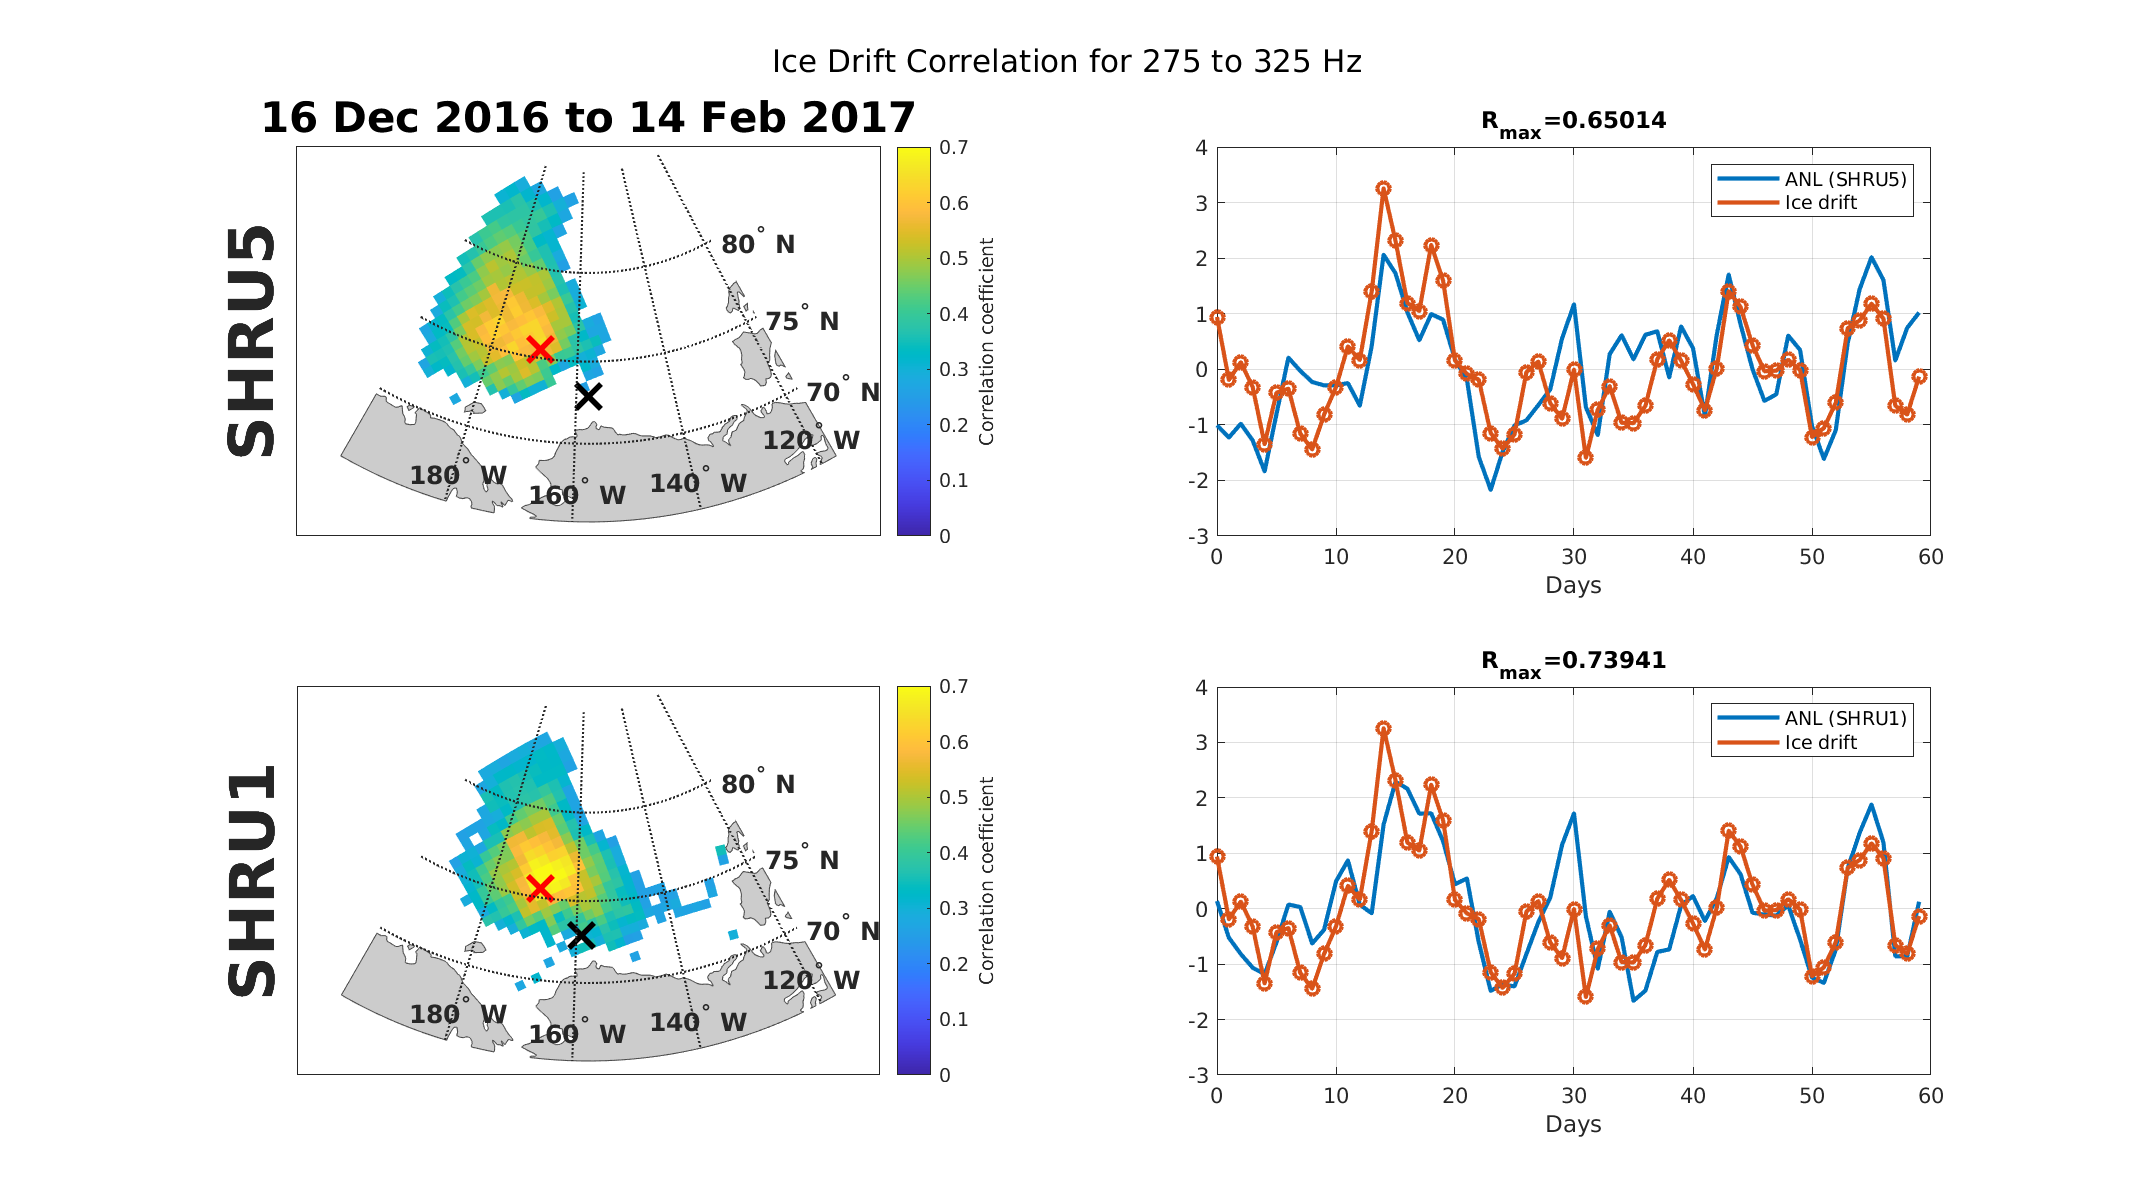
\includegraphics[scale=0.35]{Figures/300_spatial_corr_20161216-20170214_275_325.png}
\caption{Spacial Correlation map and time series for 300 Hz between SHRU1 and SHRU5 for Decmber 16, 2016 to February 14, 2017}
\label{fig_300_16DEC}
\end{figure}

\begin{figure}[p]
\centering
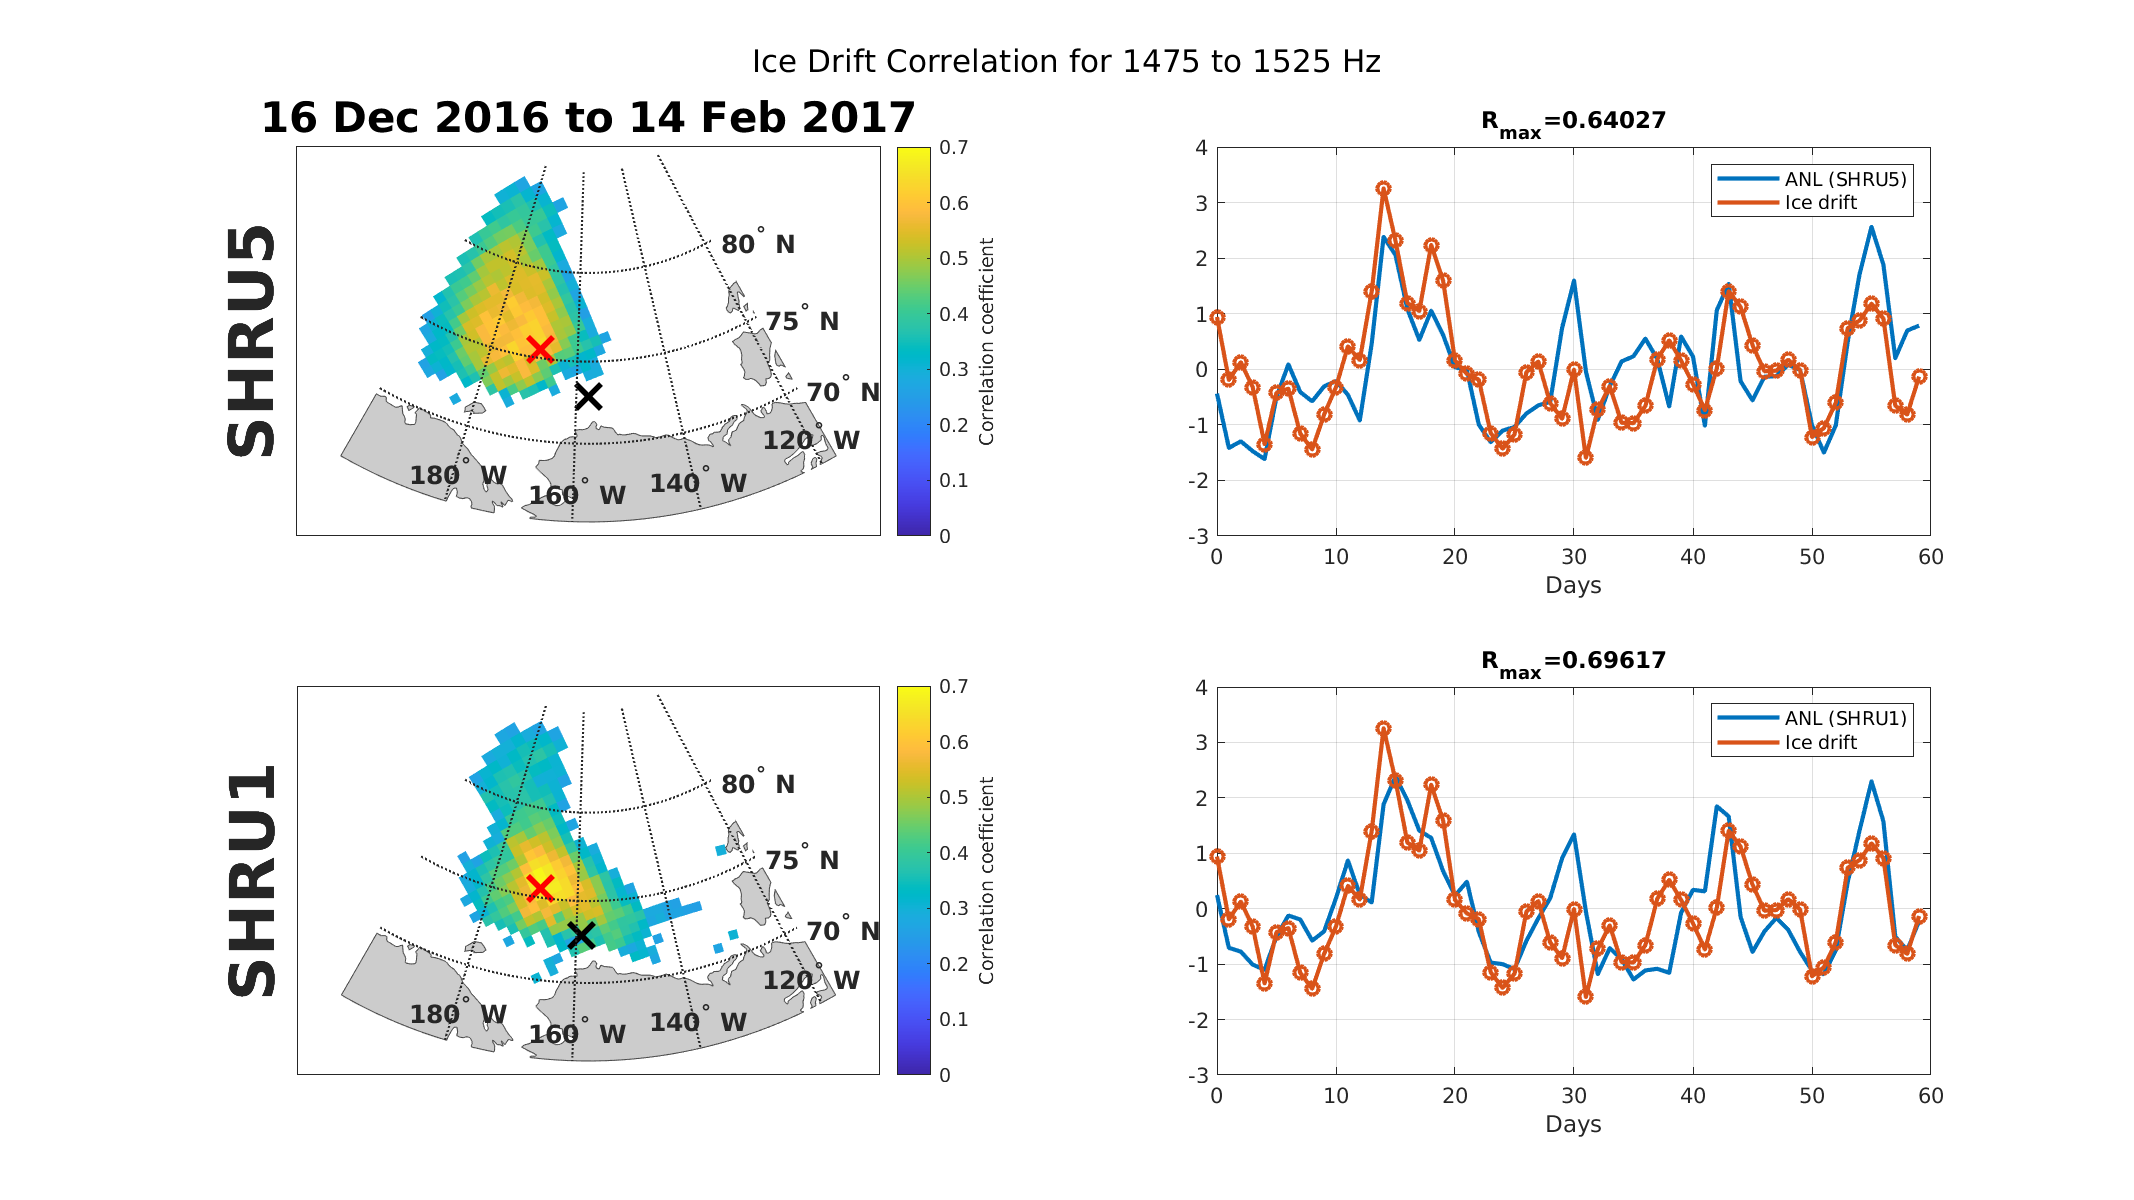
\includegraphics[scale=0.35]{Figures/1500_spatial_corr_20161216-20170214_1475_1525.png}
\caption{Spacial Correlation map and time series for 1500 Hz between SHRU1 and SHRU5 for 16DEC2016-14FEB2017}
\label{fig_1500_16DEC}
\end{figure} 

% timeseries analysis
Looking at the results for two frequencies across two hydrophones leaves no doubt that ANL and IDM are closely linked. At first glance, these two figures seem almost identical, which is beneficial for proving the hypothesis that related ambient noise caused by shared sources. A cursory observation of \autoref{fig_300_16DEC} and \autoref{fig_1500_16DEC} reveals that normalized ANL and IDM in time is virtually the same for both frequencies. Based on \autoref{fig_timeseries} and \autoref{sec_corr_freq}, normalized ANL for every frequency is almost the same when ANL oscillations aligned. Similarly, normalized IDM looks similar even if the point of maximum correlation is different for every map. Assuming the ice is essentially one interconnected sheet, especially during the winter, movement of the ice would be linked.  


%map analysis
The maps for SHRU5 and SHRU1 for 300 Hz and 1500 Hz are not the same due to the the ~50 km between the two recording units, but the area of higher correlation for all four maps is in the same general spot. As SHRU5 seems to be closer to the environmental driver, its correlation maps are tighter for both \autoref{fig_300_16DEC} and \autoref{fig_1500_16DEC}; the correlation maps for SHRU1 are a little more spread out due to extra distance and interference travelling sound would likely experience. Due to these shared attributes, the source of the noise is likely a single cryogenic driver creating most of the ambient noise during this time period. 

For the most part, oscillations in IDM and ANL at the maximum correlation coordinate match. However, there are times when increases in normalized ANL such as around day 25 do not have a corresponding increase in IDM. Some alternate source like other types of cryogenic activity \footcite[]{collins2019acoustic} or biological activity may be affecting some frequencies of the ambient sound at this time. It is interesting to note that ice is more of a distributed source or a plane source than a point source and modelling as a point source isn't entirely realistic to the environment. As Arctic ice changes with time, current, and temperature, the correlation between ANL and IDM changes as well. These changes in time will be examined further in \autoref{sec_allfreq_map}, but first this correlation trend can be examined in more frequencies.

% Note correlation tends to decrease from jan to feb, in march we lose data points for ice drift

% well its missing a title

%%%%%%%%%%%%%%%%%%%%%%%%%%%%%%%%%%%%%%%%%%%%%%%%%%%%%%%%%%%%%%%%%%%%%%%%%%
\subsection{Spatial Correlation For Frequencies in Space}  \label{sec_allfreq_map}
%%%%%%%%%%%%%%%%%%%%%%%%%%%%%%%%%%%%%%%%%%%%%%%%%%%%%%%%%%%%%%%%%%%%%%%%%%
 
\begin{figure}[p]
\centering
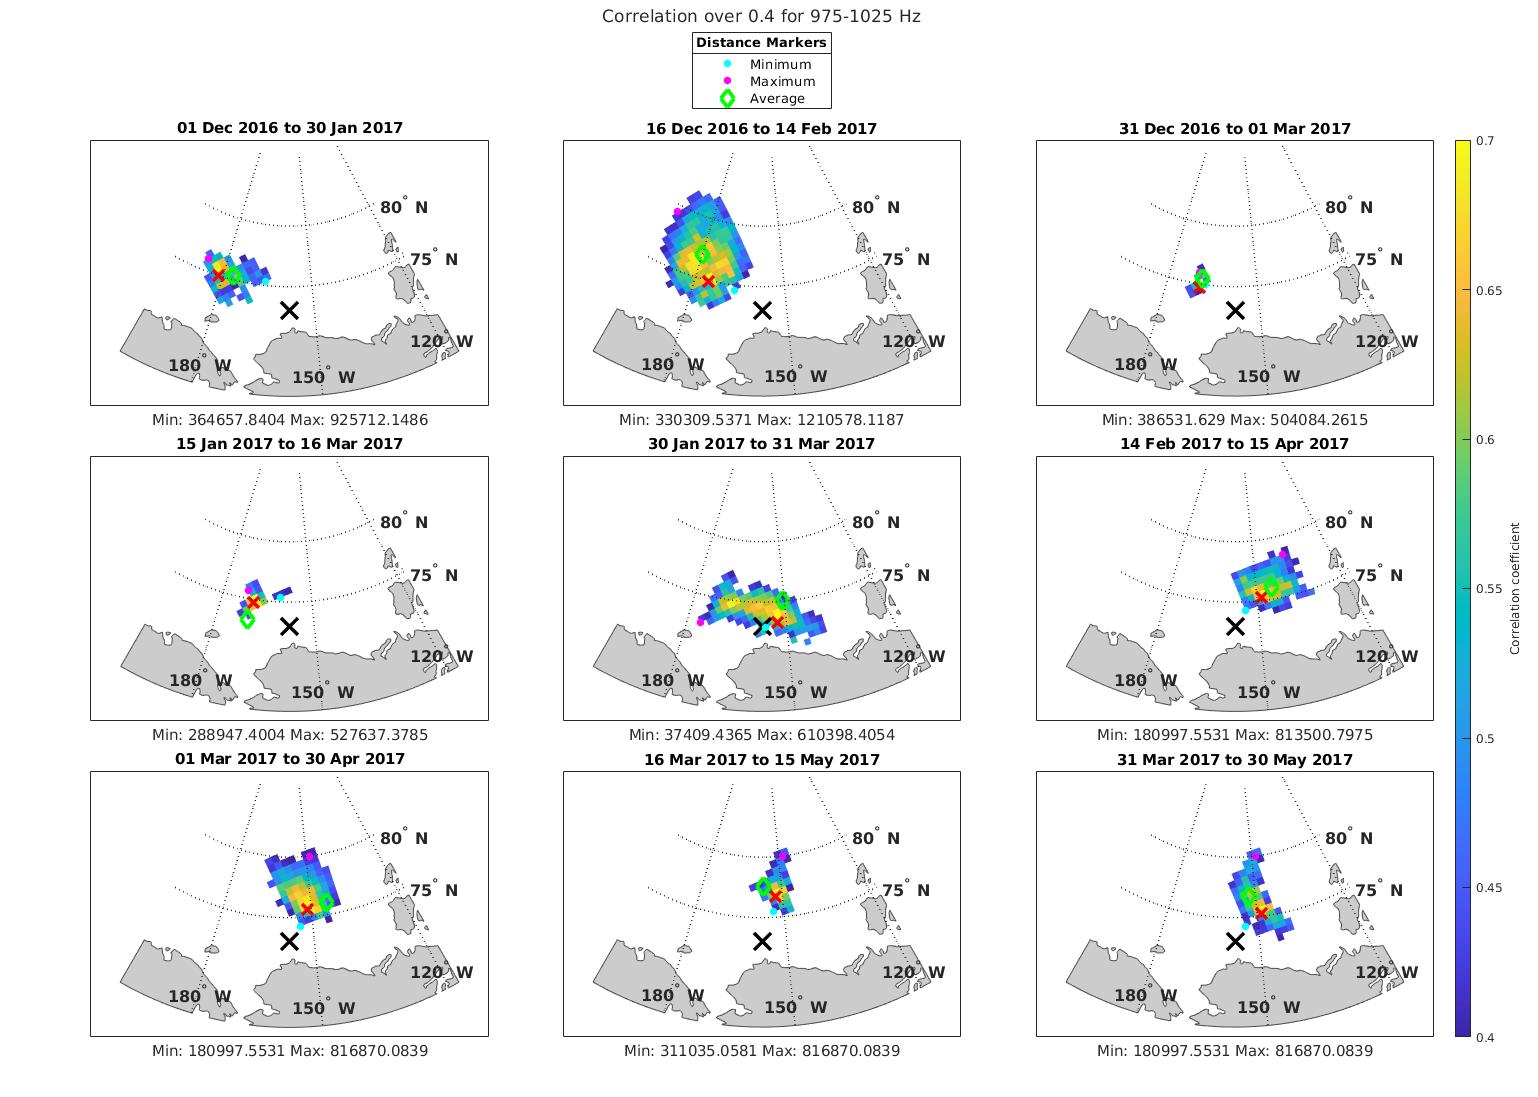
\includegraphics[scale=0.24]{Figures/megamap_noisland_0.4_1000.jpg}
\caption{Maps in time of correlation spread >0.4 for band centered on 1000 Hz with markers on minimum distance, maximum distance, and average distance. Note that the colorbar here begins at 0.4, unlike previous maps}
\label{fig_megamap}
\end{figure}

\begin{figure}[p]
\centering
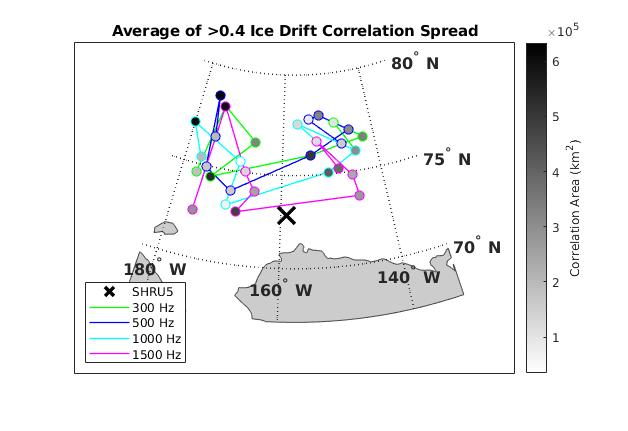
\includegraphics[scale=0.5]{Figures/avg_corr_summary.jpg}
\caption{Average point of >0.4 spatial correlation spread and area size for frequencies 300-1500 Hz}
\label{fig_avgmap}
\end{figure}

Now that a relationship between IDM and ANL is known for the frequencies of interest, analysis can be extended to look at the spread of the correlation map over time and examine the strength of the correlation as the ice changes. Taking the correlation maps from \autoref{sec_corr_shru} and \autoref{sec_corr_freq} and cutting off values $\leq 0.4$ for each time period returned new correlation matrices with more significant values. Island outliers distant from the main body of the spread were removed. For the remaining values $\geq 0.4$, the area of correlation, minimum, maximum, and average distances of the colormap were determined. \autoref{fig_megamap} shows the resulting cutoff correlation map for 1000 Hz through time. Minimum, maximum, and average markers are represented by a blue dot, pink dot, and green diamond respectively. The red X still mark the location of maximum correlation value, and the black X marks the location of SHRU5.

As anticipated, the size of the $\geq 0.4$ correlation zone in \autoref{fig_megamap} changes with time, affected by the movement of the ice sheet and other environmental factors. For all the frequencies, there is no consistent decrease or increase in size, only variations between the months. Larger correlation areas could be associated with high amounts of IDM over a large area generating sound through the ice sheet itself and into the water. Significant movement events could be a product of storms, currents, or high winds causing shifts in the ice plate. % could also be ice cracks or calving but maybe not in this particular area also not the right time for 

All the cutoff maps for 300 Hz, 500 Hz, 1000 Hz, and 1500 Hz were created and their attributes compared. The average distance location points of each frequencies were compiled into one map, shown on \autoref{fig_avgmap}. The colorfill of each average point marker represents the corresponding area of the correlation spread $\geq 0.45$ at that point. The lines of these points are connected to follow drift in time; Green is 300 Hz, blue is 500 Hz, cyan is 1000 Hz, and pink is 1500 Hz. While these points are not labelled with, the first point for every frequency begins in the west, and moves generally east. The largest correlation map areas (darkest point fill) tend to cluster in the same places at similar times, which could be large movements in the ice creating a large plane from which ambient noise emanates.

Overall there is a movement of about 1,100 km west to east of the IDM area correlating with ambient noise from SHRU5. This west to east drift in sound is a part of the polar environment affected in part by the influx of current from the Bering strait as well as the circulation of the Beaufort Gyre. Currents coming in from the Bering Sea and the Alaska Coastal Current (ACC) flow closer to the edge of land from west to east, which could affect this flow direction. \footcite[]{Weingartner2005} Interestingly, the direction of the Gyre is usually clockwise, meaning the circulation of the ice is usually east to west, opposite of the direction found in the correlation map. The area of correlation could be pushed by the ACC or sound could be generated by new ice being pushed against existing sheets. Either way, it is clear that ice drift is part of the source behind ambient noise for many frequencies during this time period. 




%%%%%%%%%%%%%%%%%%%%%%%%%%%%%%%%%%%%%%%%%%%%%%%%%%%%%%%%%%%%%%%%%%%%%%
\subsection{Distribution of Spacial Correlation through Time}
%%%%%%%%%%%%%%%%%%%%%%%%%%%%%%%%%%%%%%%%%%%%%%%%%%%%%%%%%%%%%%%%%%%%%%

Besides observing the movement of the correlation maps and average points in space, one can also compare the correlation distances in time. Another interesting metric to compare between frequencies are the distance metrics of the spread. \autoref{fig_totalice} shows the minimum, average, and maximum distance of the $\geq 0.45$ correlation spread as a series in time of errorbar-style plots for each frequency. Beginning and ending with the same date as the spacial correlation maps, these plots are a numerical approach to describing the areas where sound is correlated with IDM.Dates on the x-axis are consistent with the end two month long overlapping time period used in \autoref{sec_spa_corr_freqs}

Keeping with the same color convention of the rest of this paper, the central connected dots represent the average distance from the cutoff correlation spread. The lower and upper bounds of the bar represent the minimum and maximum distances respectively. These distance values range from just a few kilometers to over 1200 km. Similar to \autoref{fig_avgmap} the distance markers vary highly but do not follow any trends in time. 

The four subplots of \autoref{fig_totalice} show matching trends in rise and fall of average distance, but 300 Hz and 500 Hz are more similar than 1000 Hz and 1500 Hz. The length of the bars is highest for 300 Hz and decreases in size through 1500 Hz. Keeping in line with \autoref{sec_probsnstat} the larger ranges could be a result of the higher ambient noise levels experienced at low frequencies. Three of the four graphs contain a long bar during the two month period centered on February 14, 2017. When looking at the cutoff map of this time period, there is a significant point far away from the rest of the correlation spread. The maps without the correlation cutoff show a larger area of high correlation for this time period compared to the rest. This likely occurred because a large portion of ice was moving and creating sound over a wider area than other time periods.

From \autoref{fig_totalice} the similarities between the correlation of IDM and ANL frequencies over time is apparent as the distance to the source usually aligns. The distance that sound can travel under water with and without the duct is long range for more than just low frequencies. 
% this title is BAD on the figure
\begin{figure}[p]
\centering
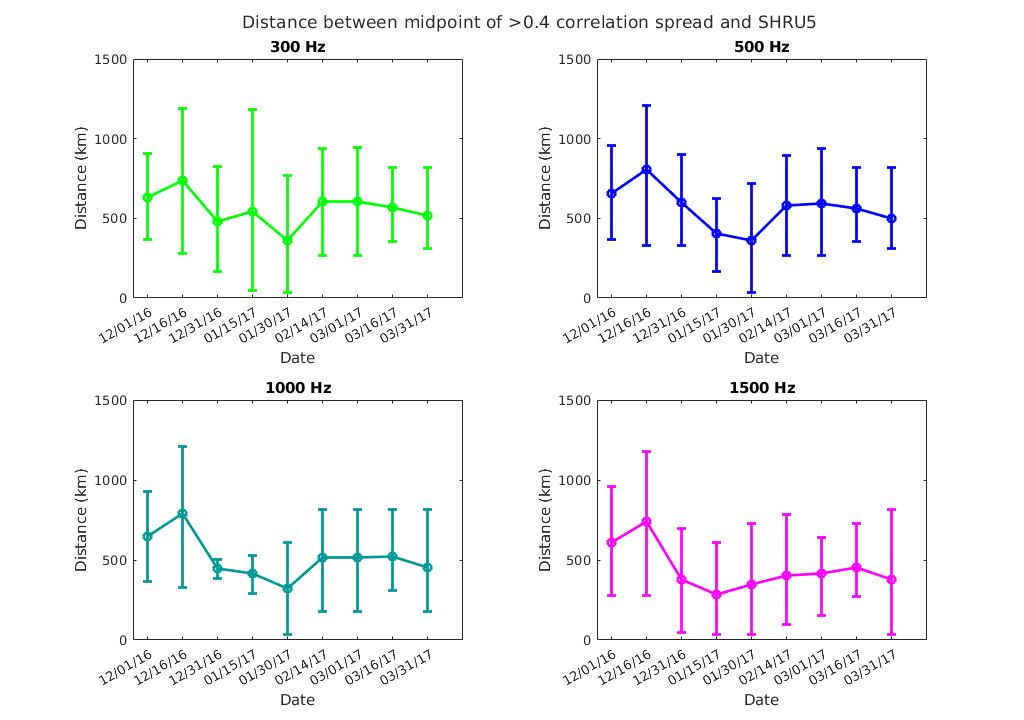
\includegraphics[scale=0.38]{Figures/errorbars_tiled_noisland.jpg}
\caption{Minimum, average, and maximum distance of the correlation spread above 0.4}
\label{fig_totalice}
\end{figure}

% btw the title on this figure is wrong fix dates and make solid lines

\begin{figure}[p]
\centering
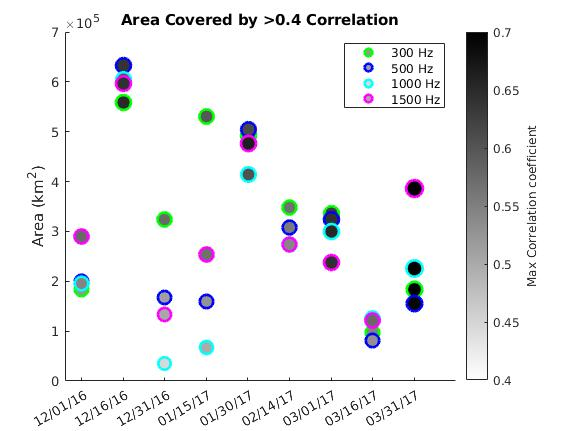
\includegraphics[scale=0.5]{Figures/area_cov_by_>0.4_noisland.jpg}
\caption{Area of correlation spread in km$^{2}$ and corresponding maximum correlation value for frequencies 300-1500 Hz}
\label{fig_maxcorr_dist}
\end{figure}

%%%%%%%%%%%%%%%%%%%%%%%%%%%%%%%%%%%%%%%%%%%%%%%%%%%%%%%%%%%%%%%%%%%%%%%%%%
%\subsection{Spacial Correlation of Frequencies through Time}
% we have combined sections 

Besides looking at the distances from the hydrophone to the correlation spread, one can also examine the area of correlation spread as it grows and shrinks through time. \autoref{fig_maxcorr_dist} shows the area of correlation spread in square kilometers, along with the maximum value of correlation at that time as the colorfill of the point. As seen in \autoref{fig_300_500corr} and \autoref{fig_1000_1500corr}, oftentimes these maximum correlation points are in very similar places, leading to overlap in the points. A coloring convention similar to \autoref{fig_totalice} is used.

The area of the correlation spread loosely decreases with time, going from around 600,000 $km^{2}$ to 200,000 $km^{2}$. The formation and shrinking of the ice pack could be responsible for the large to small correlation area differences. Interestingly, there is a pattern of alternation between a stronger and weaker correlation value. For most of the points, a higher value of correlation area coincides with a higher maximum correlation value from the spread.

Most of the points are clustered in a certain area, with an exception from December 2016 to January 2017. Most of the places where the frequencies share similar correlation areas have higher maximum correlation values as well. Continuing with the idea that large movement of large areas of sound creates higher correlation, smaller areas seem to match with lower correlation values. The four frequencies tend to have similar area and correlation values, keeping with the strong relationship between ambient noise frequencies. As these sources are wide and their initial source levels aren't known, this adds complexity to estimating the loss between the received ambient level and ice source. In order to verify many of these results, additional nontrivial modelling required. 







%%%%%%%%%%%%%%%%%%%%%%%%%%%%%%%%%%%%%%%%%%%%%%%%%%%%%%%%%%%%%%%%%%%%%%%%
\section{Spacial Analysis Conclusions} %summary? conclusion? idk what to call
%%%%%%%%%%%%%%%%%%%%%%%%%%%%%%%%%%%%%%%%%%%%%%%%%%%%%%%%%%%%%%%%%%%%%%%%

%Here, sum up the 'what does this mean of the above'
%
%\subsection{Correlation between Ice Drift and ANL}
During the Arctic winter, the Arctic ice sheet dampens most of the other ambient noise normally heard on open seas. While the acoustic environment is quieter, it is by no means silent as the ice itself becomes the primary source of ambient noise.  Whether the duct is present or not, there is significant long range travel of ambient noise associated with the drift of ice. Ambient noise is captured from these areas and correlated with the drift of ice itself. This steady correlation holds from 300 to 1500 Hz as the ambient sound permeates through all these frequencies.

The size of the correlation map and the distance from SHRU5 to this spread are also linked as a larger area of ice movement creates significant ambient noise able to travel long distances. These areas of ice drift are very large, furthering their ability to send long range sound for many kilometers. Though the size of the area, distance, and the correlation coefficients of the spread between ANL and IDM differ through time, 300, 500, 1000, and 1500 Hz change together. This further demonstrating that the ambient noise encompasses many frequencies, and is highly connected to the drift of the Arctic ice sheet. 







